\documentclass{article}
\title{Tendermint Evaluation}
\author{Simone Petruzzi-1811872 Domenico Tersigni-1817502}
\date{September 2023}
\usepackage[margin=1.5in]{geometry} % Adjust the values as per your requirements
\usepackage{amssymb}
\usepackage{amsfonts}
\usepackage{amsmath}
\usepackage{graphicx}
\graphicspath{ {./images/} }
\usepackage{xcolor}
\usepackage{listings}
\lstdefinestyle{bashstyle}{
    language=Bash,
    basicstyle=\ttfamily,
    keywordstyle=\color{blue},
    commentstyle=\color{green!40!black},
    numbers=left,
    numberstyle=\tiny,
    numbersep=5pt,
    frame=single,
    breaklines=true,
    breakatwhitespace=true,
    tabsize=4
}

\begin{document}
   \maketitle
   \section{Introduction}
  Consensus is one of the most fundamental problems in distributed computing. It is importante because of its role in State Machine Replication (SMR), an approach for replicating services. The key idea of this approach is that service replicas start in the same initial state and then execute transactions in the same order. Consensus is the way for ensuring that all replicas receive transactions in the same order.
Traditionally, deployments of SMR based systems are in data-center settings (LAN), where there are a small number of replicas and they are typically part of a single administration domain. In this scenario Byzantine faults can be neglected. 

In recent years the problem has attracted more significant attention due to the widespread success of blockchain-based digital currencies such as Bitcoin and Ethereum. In this scenario, SMR based systems should reach agreement over Wide Area Network (WAN), where there are a large number of nodes that are not part of the same administration domain. It is easy to understand that in this setting a subset of nodes can behave maliciously and the probability of Byzantine faults is no more negligible.
Furthermore, nodes are not fully connected to each other, but a node is only connected to a subset of other nodes (called peers) and the communication among all nodes is achieved by gossip-based peer-to-peer protocols.
\newline
\newline
The Tendermint platform consists of a high-performance Byzantine Fault Tolerant (BFT) SMR implementation, written in Go, which is a flexible interface for building deterministic applications above the consensus.  We focus on a BFT consensus algorithm that is the core of the Tendermint platform. 

   \subsection{Model}
   Focusing on SMR based systems over WAN, we consider a system of processes that communicate by exchanging messages, processes can be correct or faulty and we consider Byzantine faults. Furthermore, we assume that each process has some amount of voting power (voting power of a process can be 0). We model network communication through a modified version of the partially synchronized system model, in which we have an upper time bound $\Delta$ and an instant called GST (Global Stabilization Time) such that all  communication among correct processes after this time is reliable and $\Delta$-timely. In addition to the standard partially synchronized system model we assume an auxiliary property that captures gossip-based nature of communication:
\begin{itemize}
\item Gossip communication: If a correct process p sends some message m at timet, all correct processes will receive m before max$\{t,GST\} $+ $\Delta$. Furthemore, if a correct process p receives some message m at time t, all correct processes will receive m before max$\{t,GST\}$ + $\Delta$.
\end{itemize}
  We assume that process steps like sending and receiving messages take zero time and that processes are equipped with clocks so they can measure local timeouts. Spoofing attacks are not possible due to public-key cryptography, infact we assume that all messages are digitally signed.

   \subsection{State Machine replication}
 The most important property for SMR is: 
   \begin{itemize}
   	\item Replica coordination: all non-faulty replicas receive and process the same sequence of requests.
   \end{itemize}
 This property can be decomposed in two parts: Agreement and Order. 
Agreement means that all non faulty replicas receive all requests, and Order requires that the order of received requests is the same at all replicas.
It is important to stress that only requests proposed by clients are executed. In Tendermint, transaction verification is the responsability of the service that is being replicated, upon receiving a transaction from the client, the Tendermint process will ask the service if the requests is vaid, and only valid requests will be processed.
  
   \subsection{Consensus}
   Tendermint solves the state machine replication problem by sequentially executing consensus instances to agree on each block of transaction that are executed by the service being replicated. This problem is define by the following poperties:
   \begin{itemize}
   	\item \textbf{Agreement}: No two correct processes decide on different values.
	\item \textbf{Termination}: All correct processes eventually decide on a value.
	\item \textbf{Validity}: A decided value is valid, i.e., it satisfies the predefined predicate denoted valid().
   \end{itemize}
   \newpage
   \section{Tendermint consensus algorithm}
   We assume that there is a gossip-based protocol for disseminating messages, and every process stores messages in a local message log for every process. The algorithm is presented as a set of upon rules that are triggered once the message log contains messages such that the corresponding condition evaluates to true. \\
   The algorithm proceeds in rounds, each of it having a dedicated proposer. Processes are all aware of the rounds by simply processing the $propose(h,round)$ function, that returns the proposer for the $round$ in the consensus instance $h$. In each round of consensus, one validator is selected as the proposer through a weighted round robin function, where processes are rotated proportional to their voting power.\\ \\
	Processes in Tendermint exchange three types of messages: PROPOSAL, PREVOTE, PRECOMMIT. Thus Tendermint, requires two voting steps (three communication exchanges of messages in total). The PROPOSAL message is the only carrying the value $v$ (in this context a block of transactions) and a value id, PREVOTE and PRECOMMIT carry only the value id. A correct process decides a value $v$ after having received $2f+1$ voting power equivalent PRECOMMIT messages for it. In order to send PRECOMMIT for some messge $v$ in a round $r$ a process must wait for the PROPOSAL and $2f+1$ of the corresponding PREVOTE messages in the round $r$. Otherwise it sends PRECOMMIT message with a special $nil$ value (ensuring that corrects can PRECOMMIT only a single value in a round). Since proposers may be faulty , the proposed value is treated by corrects like a suggestion, and corrects tell each others if they accepted the PROPOSAL for a certain value by sending PREVOTE message for it. Otherwise like for the PRECOMMIT message, it sends PREVOTE message with a $nil$ value. \\ \\
	Every process mantain the following variables: $step$, $lockedValue$, $lockedRound$, $validValue$ and $validRound$. The $step$ denotes the stage of the algorithm execution in the current round. $lockedValue$ holds the latest value sent with a PRECOMMIT message for a specific round number, and $lockedRound$ is the last round with a non-$nil$ PRECOMMIT message. A correct process locks a value $v$ in round r by setting $lockedValue$ = $v$ and $lockedRound$ = r before sending a PRECOMMIT message for id(v). To make a decision, a correct process needs 2f + 1 PRECOMMIT messages for id(v), meaning a possible decision value is locked by at least f + 1 voting power equivalent of correct processes. Thus, any value v receiving PROPOSAL and 2f + 1 corresponding PREVOTE messages in round r is a possible decision value. $validValue$ stores the most recent possible decision value, and $validRound$ is the last round it was updated. Additionally, each process stores its current consensus instance ($h_p$ or height in Tendermint) and the current round number ($round_p$) attached to every message. Finally, a process maintains an array of decisions, $decision_p$, for each consensus instance. \\ \\	
	Each round starts with a proposer using a PROPOSAL message to suggest a value. In the first round of each height, the proposer can freely choose the suggested value. A correct process gets a proposal value using the external function $getValue()$, ensuring it's valid. In subsequent rounds, a correct proposer only suggests a new value if $validValue$ is $nil$. Otherwise, $validValue$ is proposed. The PROPOSAL message includes $validRound$ to inform others of the last round where $validValue$ was considered a possible decision. If a correct process $p$ sends $validValue$ with $validRound$ in the PROPOSAL, it means $p$ received PROPOSAL and the corresponding $2f + 1$ PREVOTE messages for $validValue$ in $validRound$. When a correct process sends a PROPOSAL message with $validValue$ ($validRound > -1$) at time t $>$ GST, gossip communication ensures all correct processes receive the PROPOSAL and PREVOTE messages before $t + \Delta$. Thus, they can verify the suggested value's correctness, supported by the PROPOSAL and 2f + 1 equivalent voting power PREVOTE messages. \\ \\
	A correct process $p$ accepts a proposal for value $v$ (i,e. sends PREVOTE for $id(v)$) if an external valid function approves $v$, and if $p$ has not locked any value ($lockedRound = -1 $) or has locked value $v$ ($lockedValue = v$). If the proposed pair is (v, vr $\geq$ 0), and a correct process p has already locked a value, it will accept v if it's a more recent possible decision value ($v_r > lockedRound_p$) or if $lockedValue = v$. Otherwise, a correct process rejects the proposal by sending a PREVOTE message with a nil value. Additionally, a correct process sends a PREVOTE message with a nil value if the $timeoutPropose$ has expired (triggered when a correct process starts a new round) and the process hasn't sent a PREVOTE message in the current round yet.\\ \\
	When a correct accepts a proposal for a value $v$ by sending a PRECOMMIT message with $id(v)$ if it receives a PROPOSAL message for $v$ along with 2f + 1 PREVOTE messages for $id(v$). Otherwise, it sends a PRECOMMIT message with a nil value. In the event that a correct process hasn't sent a PRECOMMIT message in the current round and the $timeoutPrevote$ has expired, it will also send a PRECOMMIT message with a nil value.To make a decision, a correct process requires receiving a PROPOSAL message for a value $v$ in some round $r$ and requires receiving also 2f + 1 PRECOMMIT messages referencing id(v). To prevent the algorithm from becoming stuck indefinitely,it is used $timeoutPrecommit$, which triggers after a process receives any set of 2f + 1 PRECOMMIT messages for the current round. If the $timeoutPrecommit$ expires and a process hasn't made a decision yet, it initiates the next round. Upon reaching a decision, a correct process $P$ initiates the next consensus instance for the subsequent height. The Gossip communication property ensures that the PROPOSAL and 2f + 1 PREVOTE messages that led $p$ to make a decision will eventually be received by all correct processes, facilitating their own decision-making process.
	\subsection{Termination mechanism}
	Tendermint ensures termination by a novel mechanism that benefits from the gossip based nature of communication. This is possible thanks to the variables validValue and validRound mentioned above. Let's see briefly the intuition how managing and proposing these two variables ensures termination. 
We can have three possible scenarios:
\begin{itemize}
	 	\item During good period, beacuse of Gossip communication property, if a correct process p locks a value v in some round r, all correct processes will update validValue to v and validRound to r before the end of the round r. The intuition is that messages that led to p locking a value v in the round r will be gossiped to all correct processes before the end of the round r, so they will update validValue and validRound. Therefore, if a correct process locks some value during good period, validValue and validRound are updated by all correct processes, so the value proposed in the following rounds will be acceptable by all correct processes.
	 	\item It could happen that during good
period, no correct process locks a value, but some correct process q updates validValue and validRound during some round. As no correct process locks a value in this case, validValue of q and validRound of q will also be acceptable by all correct processes as validRound of q $>$ lockedRound of c for every correct process c and as the Gossip communication property ensures that the corresponding PREVOTE messages that q received in the round validRound of q are received by all correct processes $\Delta$ time later.
          \item Finally, it could happen that after GST, there is a long sequence of rounds in which no correct process neither locks a value nor update validValue and validRound. In this case, during this sequence of rounds, the proposed value suggested by correct processes was not accepted by all correct processes. Note that this sequence of rounds is always finite as at the beginning of every round there is at least a single correct process c such that validValue of c and validRound of c are acceptable by every correct process. This is true as there exists a correct process c such that for every other correct process p, validRound of c $>$ lockedRound of p or validValue of c = lockedValue of p. This is true as c is the process that has locked a value in the most recent round among all correct processes (or no correct process locked any value). Therefore, eventually c will be the proper in some round and the proposed value will be accepted by all correct processes, terminating therefore this sequence of rounds.
	\end{itemize}
Note that this mechanism does not require exchanging any additional information in addition to messages already sent.
	\newpage
	\newpage
	\section{Tendermint}
	Now that we talked about the consensus algorithm, let's talk about Tendermint in general. Tendermint is basically two things:
	\begin{itemize}
	 	\item Tendermint Core
	 	\item Application Block Chain Interface (ABCI)
	\end{itemize}
	\subsection{Tendermint Core}
	Tendermint Core is the actual consensus engine, and protocol. It works like practical Byzantine fault tolerant, with rotating leaders. It tolerates up to $\frac{1}{3}$ nodes failing. This is a proof of stake (PoS) protocol, thus there is no mining and validators as previously said, may not have equal voting power.
	\subsection{ABCI}
	This is the interface that allows your app to communicate with Tendermint Core and ensures that the app is properly replicated across all correct nodes in the network. The application must be deterministic. It must implement few methods:
	\paragraph{CheckTx}
	The check transaction method is responsible for checking that a transaction is properly formatted, has correct signature and more in general that it conforms to the protocol. This is the only method that receives transactions before consensus has been run on them. Thus this method should not modify the application state at all.
	\paragraph{DeliverTx}
	The deliver transaction is the method that takes a transaction and modifies the application state (eg: change account balance). This method is called for each transaction in a block and then commit is called.
	\paragraph{Commit}
	This method persist the application state and is responsible for computing the hash of the application state and returning it. This hash can lately be used to validate queries.
	\paragraph{Query}
	This method is used to query a piece of the application state (eg. balance of a single account). Ideally it should include some kind of proof that the piece of the application state it is returning, belongs to a certain application state within an application hash. \\
	\begin{figure}[htbp]
    \centering
    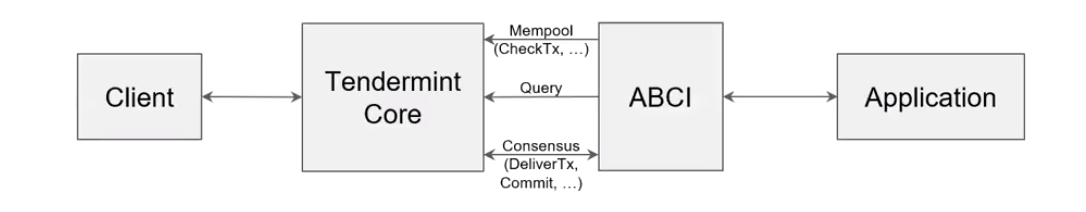
\includegraphics[width=1\textwidth]{im1} 
    \caption{architecture}
	\end{figure}\\
    Let's see in general, how a system based on Tendermint works. Users in the system submit transactions to a certain node, and those transactions first run into the application CheckTx method. In case the transaction doesn't pass the check, it will be handled by the application. If instead, the transaction is valid, it is sent to the mempool, attending for being included in a block. When a validator proposes a new block, it selects some transactions from its mempool, perhaps even prioritizing some over others, based on some conditions. At this point, three rounds of voting occur. The block is broadcasted to all validators and each votes on wether or not the block is valid. They broadcast their vote to the rest of the network (usually nodes are interconnected to a subset of the node set) and wait for $\frac{2}{3}$ of the nodes to respond with their votes. If more than $\frac{2}{3}$ of the validators respond with a positive PREVOTE, then every correct node broadcasts a positive PRECOMMIT, wheter or not it voted positively in the PREVOTE round. Finally a validator receives PRECOMMITS from $\frac{2}{3}$ of the validators, then it commits the block to the chain and begins running transactions through your application's implemented methods.
	\begin{figure}[htbp]
    \centering
    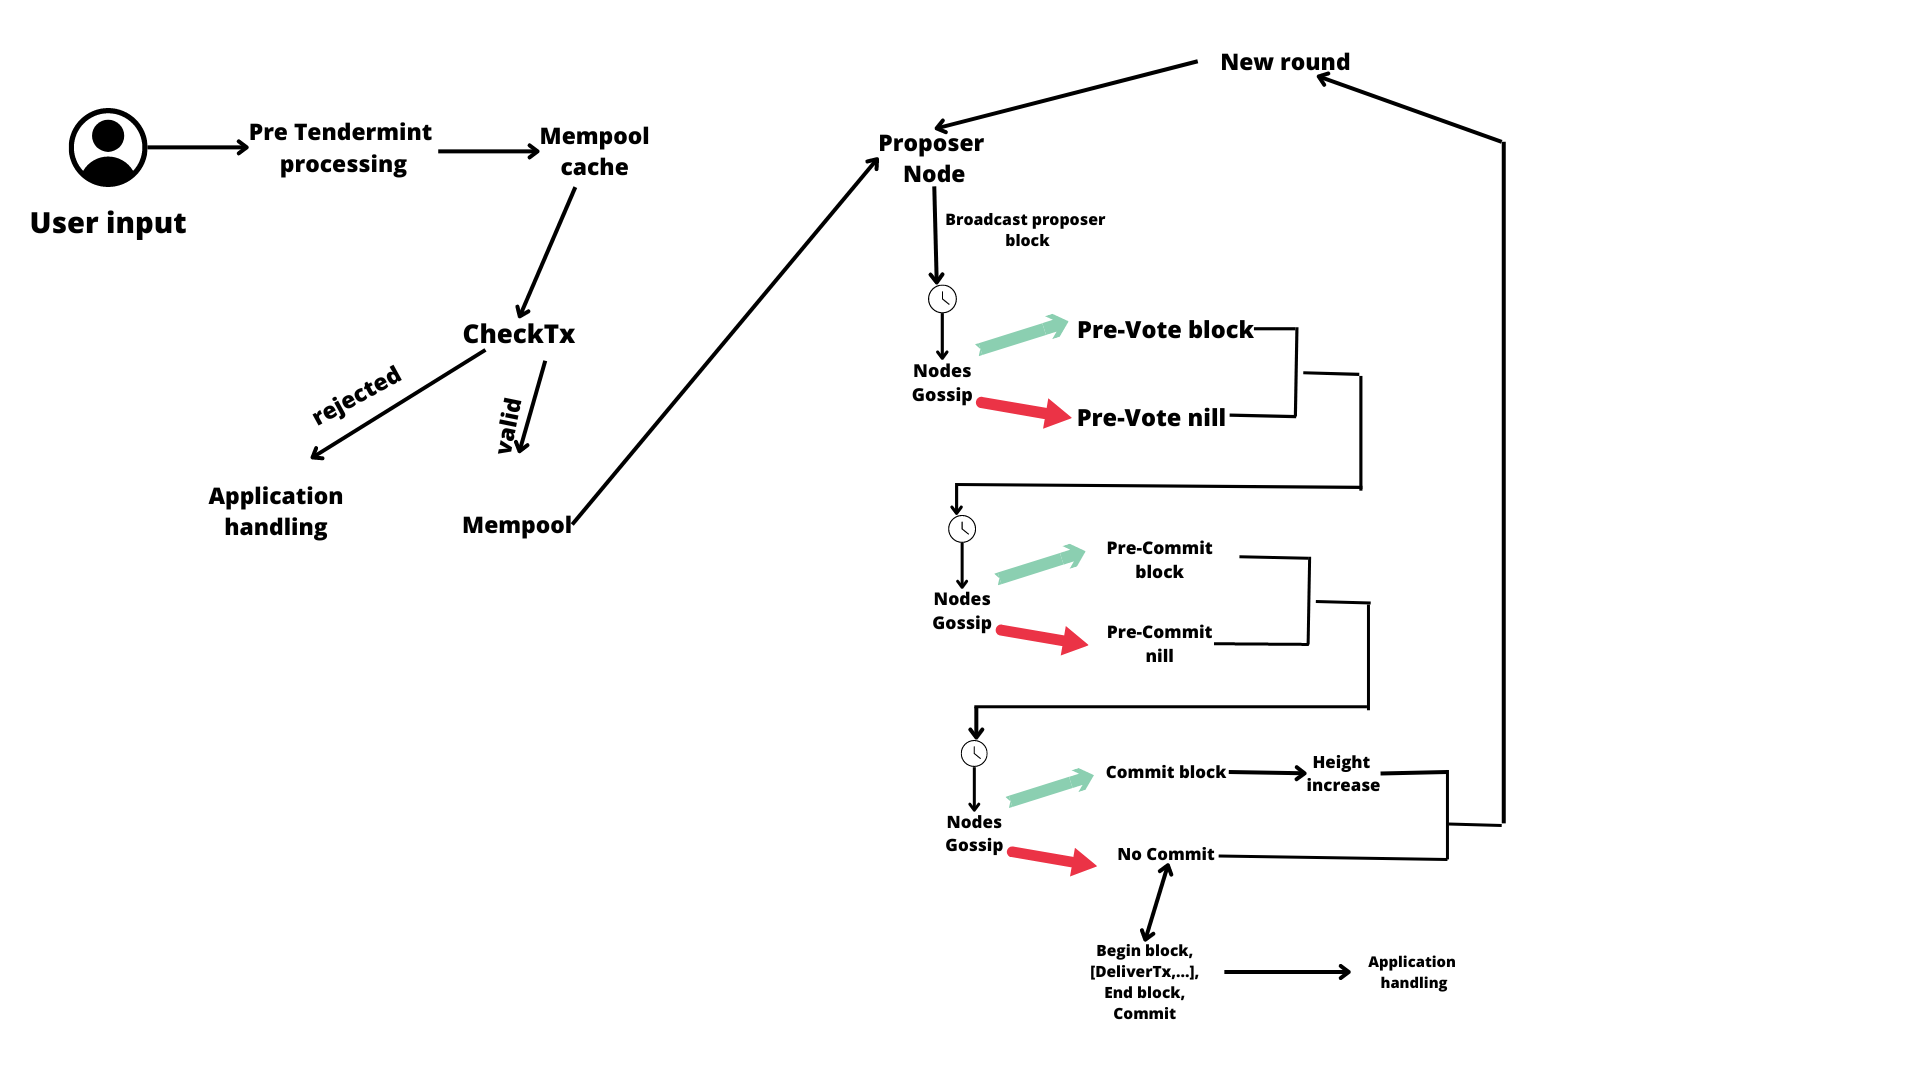
\includegraphics[width=1\textwidth]{Userinput} 
	\caption{Tendermint in a nutshell}
	\end{figure}\\
\newpage
	\section{Experiments}
	\subsection{Implementation choices and potential limitations}
	At this point let's switch to experiments we did on Tendermint. First of all we discuss briefly the implementations choices. We did those experiments on Tendermint 0.34.24 version, using docker to simulate a network of validators that run the consensus algorithm. The operating system on which we have built our experiments is Ubuntu 22.04. This set up obviously is not ideal for testing a real system, since we have that all nodes run in a local machine, we can not simulate real network. Indeed in this scenario, links work at full speed continuously, never experiencing slowdown. Also we must consider the fact that the machines on which we did the experiments are laptops with limited computational power. Both of us are equipped with a 4 core processor, therefore we thaught that was not useful to do testing on networks composed by more than 4 validators nodes.
	\subsection{Functionality analysis}
	Once we set up Tendermint running with Docker, we started to test the basic functionalities. The ABCI implemented is a simple key-value store application, it simply stores in blocks transactions that are proposed by clients (in this case a simple command line through wich we submit transactions and query the blockchain to check if they are inserted). \\ \\ 
	First of all we start by checking the status of the application by inserting in a terminal the following command:
	\begin{lstlisting}[style=bashstyle]
	curl -s localhost:26657/status
	\end{lstlisting}
	when, the application is running it responds with a message in JSON format which includes a lot of information like: the protocol version, the address and port on which the application is running, latest blockchain height, latest blockchain time, hash of the last block and many others. \\
	We can also query the status of the chain and searching for specific field and not returning the whole status, in the following example we ask for $latest_app_hash$ in particular.
	\begin{lstlisting}[style=bashstyle]
	curl http://localhost:26657/status | json_pp | grep latest_app_hash	
	\end{lstlisting}
	When the key-value store app is running we can start sending transactions with the following command:
	\begin{lstlisting}[style=bashstyle]
	curl -s 'localhost:26657/broadcast_tx_commit?tx="abcd"'
	\end{lstlisting}
	When a transaction is sent to a Tendermint node, it will run via CheckTx against the application. If it passes CheckTx, it will be included in the mempool, broadcasted to other peers, and eventually included in a block.
	We can use the following command to check if the transaction reached the validators and is inserted in the block chain:
	\begin{lstlisting}[style=bashstyle]
	curl -s 'localhost:26657/abci_query?data="abcd"'
	\end{lstlisting}
	We can also decide to send transactions with a key value too:
	\begin{lstlisting}[style=bashstyle]
	curl -s 'localhost:26657/broadcast_tx_commit?tx="name=xxx"'
	\end{lstlisting}
	and then query the key to get back the value in hexadecimal format:
	\begin{lstlisting}[style=bashstyle]
	curl -s 'localhost:26657/abci_query?data="name"'
	\end{lstlisting}
	Everytime Tendermint starts, if a blockchain exists, it will take some time before starting for reading and loading all the existing blockchain. Once the blockchain is read Tendermint starts to run consensus and produce blocks. If we want to start a brand new chain and reset the old one, stop the nodes and run:
	\begin{lstlisting}[style=bashstyle]
	tendermint unsafe_reset_all
	\end{lstlisting}
	This command will remove the data directory and reset private validator and address book files.\\
\newline
	To start a testnet composed by 4 nodes (validators) we have to open a terminal, go to the path where Tendermint is and run the following commands:
	\begin{lstlisting}[style=bashstyle]
	make build-linux   
	make localnet-start 
	\end{lstlisting}
	at this point nodes are created and successfully running. The nodes bind their RPC servers to ports 26657, 26660, 26662, and 26664 on the host.
The nodes of the network expose their P2P and RPC endpoints to the host machine on ports 26656-26657, 26659-26660, 26661-26662, and 26663-26664 respectively.\\
\newline
During the running of the testnet, we tested the resistance of our network to node failures. We could observe that killing a single node did not affect at all the correctness of the network. If instead, we stop in Docker two nodes, the consensus stops (the other two nodes alive are stucked into the reconnection procedure with the stopped peers) and we can not anymore process any transaction and no more blocks are added to the chain. If we are able to reconnect a node to the network, we will see that the node at first reconstructs the chain by reading it from file (every node/container has its own storage file for the chain), then it queries the other nodes for adding possibly missing blocks and eventually the consensus process restarts.
	
	\subsection{Tools}
	In order to analyze and carry out a performance evaluation, we made use of tools provided in Tendermint official documentation. In order to collect metrics we enabled the metrics exposure on a specific port on localhost (26666) and then collected periodically with Prometheus tool. Using prometheus we were able to monitor a lot of parameters over time and see how they evolved. Tendermint exposes a lot of interesting metrics such as: number of transactions per second, block size, consensus height and many others (please refer to official documentation to check them). \\ \\
	Also we used $tm-load-test$ tool, this is a distributed load testing tool (and framework) for load testing Tendermint networks. We used it in standalone mode for generating transactions during a specified time window, and sending to nodes of our networks.
	\subsection{Results}
During our analysis we could collect some interesting informations. First of all we tested the fault tolerance; let's recall that our test network is composed by four nodes, thus to let it work, we need at least three nodes running. The test was successfull, indeed, as we can see from the below charts built with Prometheus, until the four nodes where all active, the consensus was running, transactions were processed and put in blocks. At a given moment we shut down two nodes and we could experience the stop of the algorithm.
 	\begin{figure}[htbp]
    \centering
    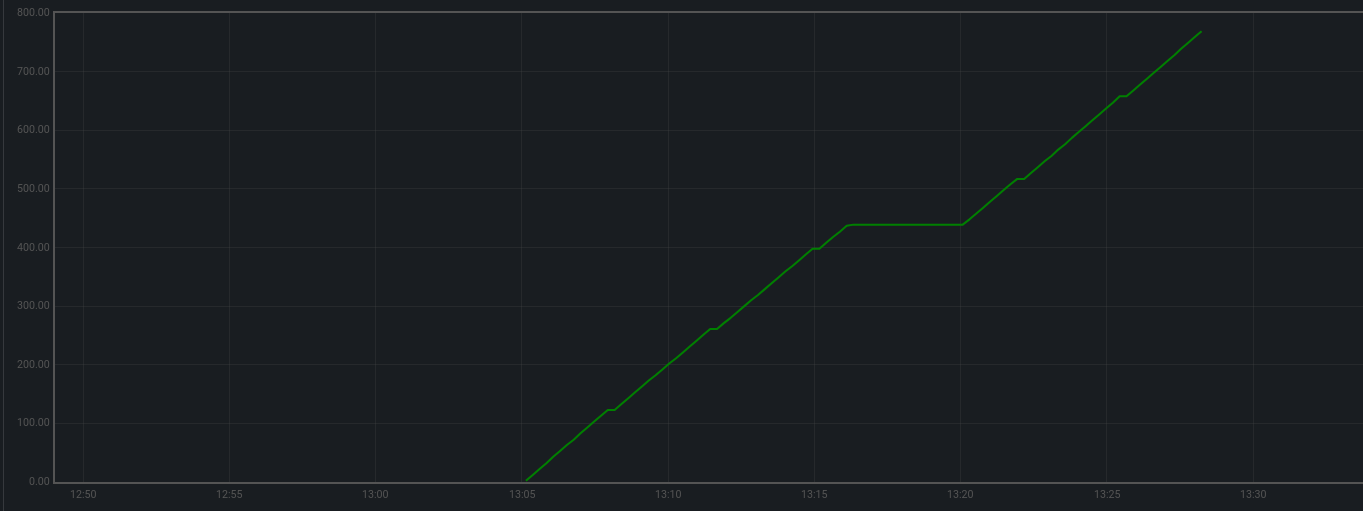
\includegraphics[width=1\textwidth]{block_count} 
	\caption{Number of blocks written over time}
	\end{figure}\\
	\begin{figure}[htbp]
    \centering
    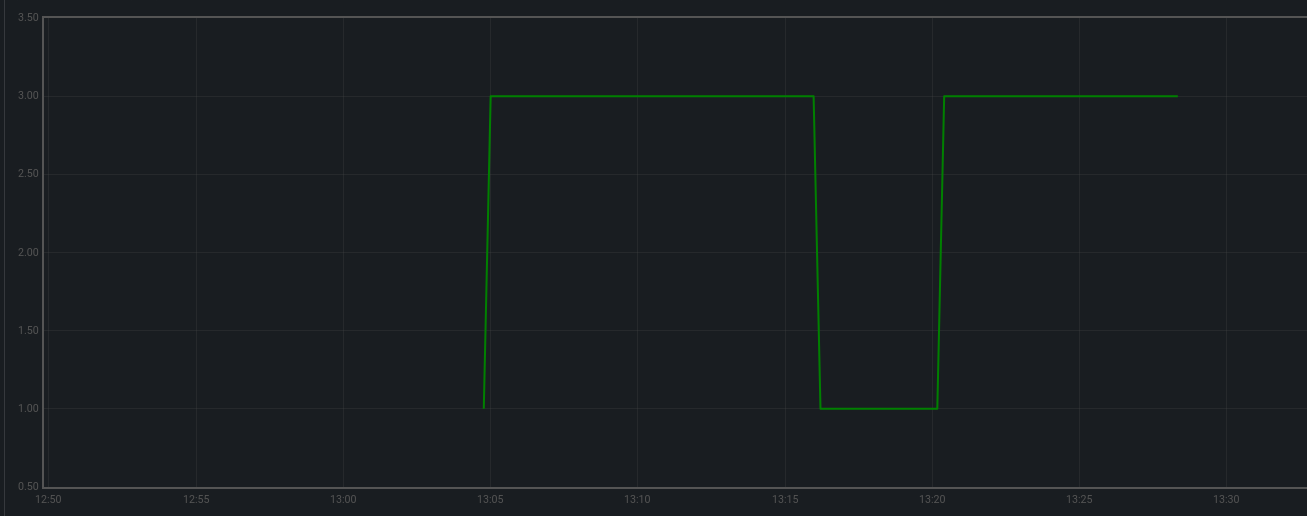
\includegraphics[width=1\textwidth]{peers_active} 
	\caption{Peers active over time}
	\end{figure}\\
	From the two figures it is really clear to note the stop of block processing. In correspondence of time $13:16$, two peers were stopped and as we can see from Figure3, the number of blocks processed remains constant, indicating that the two nodes left up stopped the consensus. Once the two nodes are restarted at time $13:21$, the whole consensus restarts, and blocks are produced at more or less the same rate as before. During this stop period, transactions are received by the two working nodes and put in the mempool without being included in new blocks. As we can see in Figure 5, during the stop time, the mempool size increases a lot, and when the nodes restart, transactions inside of the mempool are processed and included in new blocks. During this test we injected for a time period of 25 minutes more or less, 600000 transactions over two validators (300000 for each validator). Total bytes written are 89900000 bytes for an average transaction rate of 350 transactions per second.
	\begin{figure}[htbp]
    \centering
    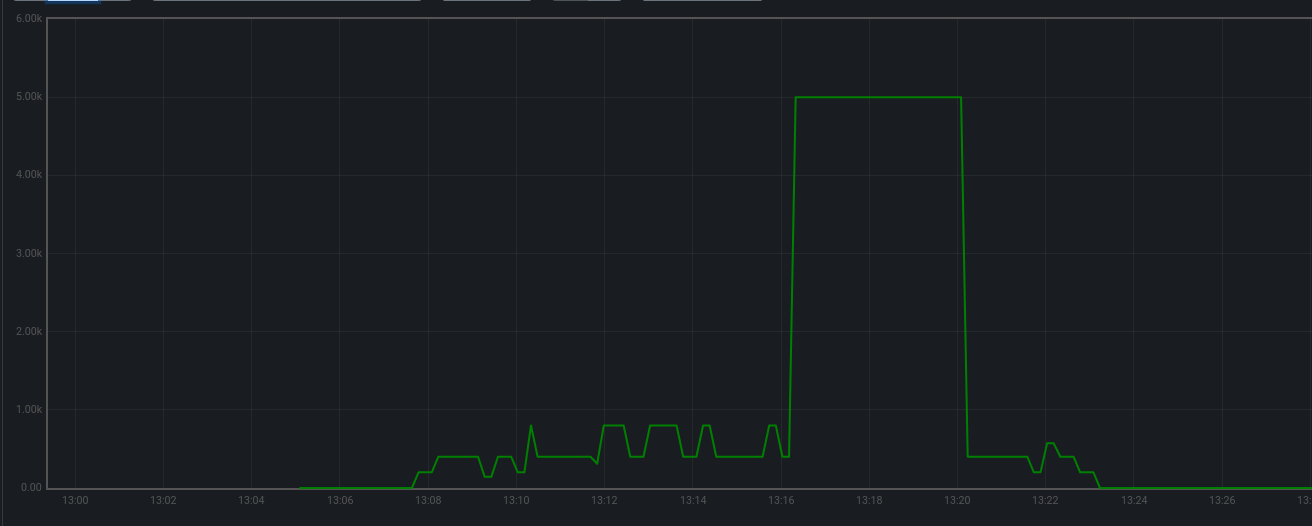
\includegraphics[width=1\textwidth]{mempoolsize} 
	\caption{Mempool size over time}
	\end{figure}\\
	We tried also to carry out a performance evaluation, finding that a network composed by four validator is more powerful than a network composed by three validators. The first parameter we took under consideration regards blocks written over time. As we can clearly see in Figure6 at time $15:40$, line slope decreases, this is due to the fact that the fourth node has been turned off.
	\begin{figure}[htbp]
    \centering
    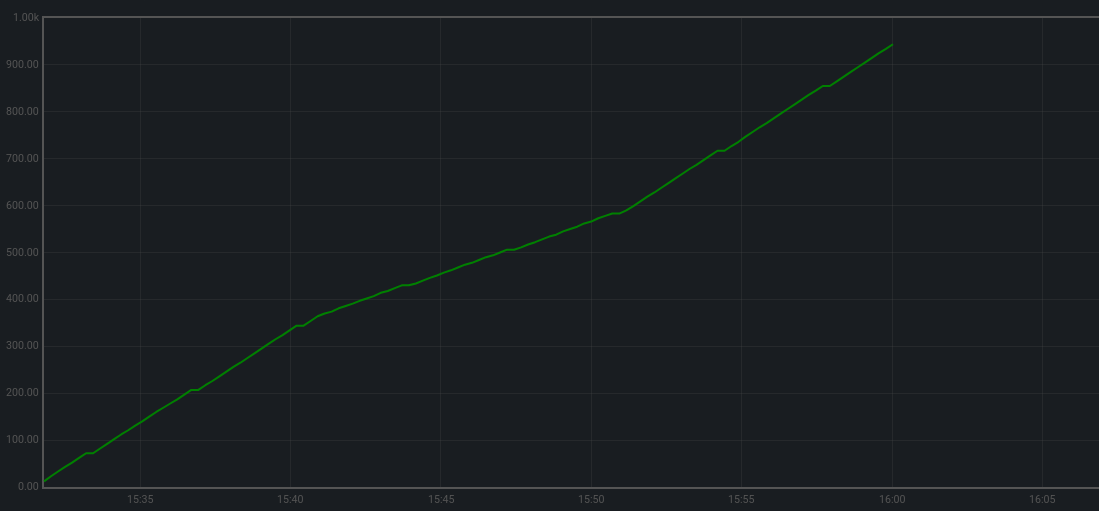
\includegraphics[width=1\textwidth]{block_count2} 
	\caption{Number of blocks written over time}
	\end{figure}\\
	When, at time $15:52$ the fourth node is restarted, we can see the slope increasing to the same as before. We can clearly see the node stopping in the Figure 7.
	\begin{figure}[htbp]
    \centering
    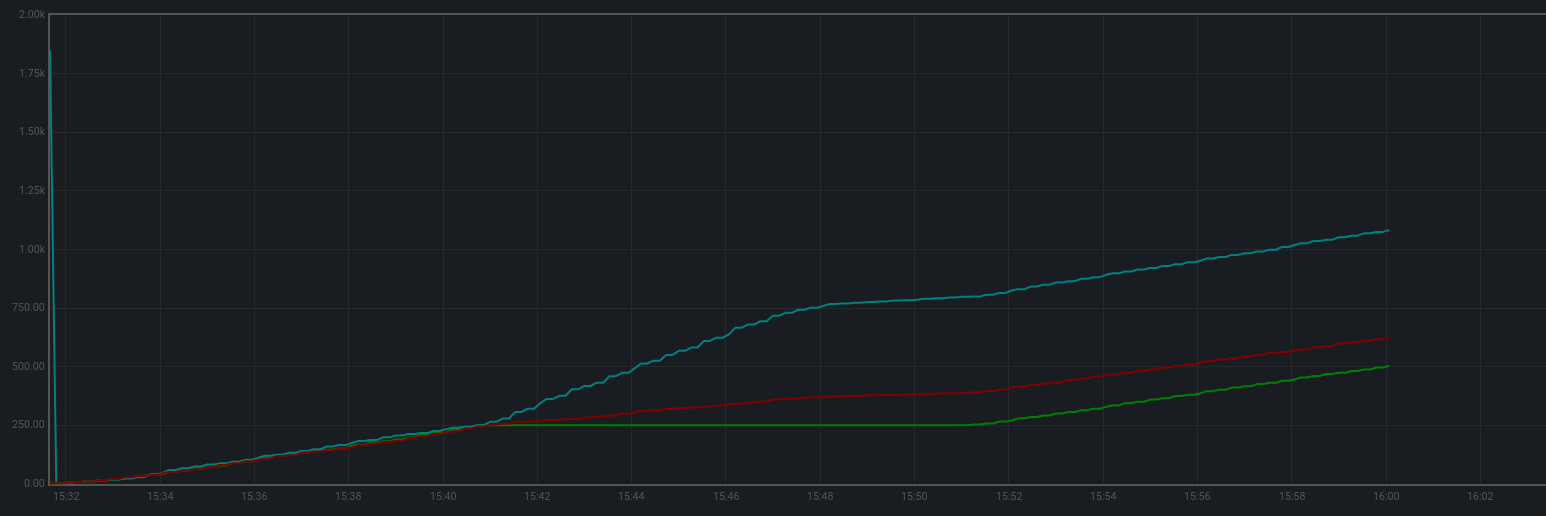
\includegraphics[width=1\textwidth]{peers} 
	\caption{Peers status}
	\end{figure}\\
	\section{Conclusion and future works}
	Although this study is not very interesting from the practical point of view, since it is build in a scenario where a lot of contraints are not considered, it can be considered as an initial step to go through distributed systems and their algorithms. We could prove the fault tolerance of the Tendermint algorithm and also the performance depending on the number of nodes partecipating to the network. \\ \\
	As future work, would be very interesting to deploy Tendermint on different machines, placed on different networks and see how the latency could affect the computation and performance. This could be done for example by exploiting the various cloud services like AWS or Azure.
\end{document}